\section{Теории: интуиция}

В этом пункте мы попытаемся на очень неформальном интуитивном уровне понять, в чем состоят базовые вопросы логики и откуда они возникают при рассмотрении математических теорий, которые, на первый взгляд, не имеют непосредственного отношения к логике. Это будет очень неформальный материал, и я заранее должен оговориться, что подходы и определения, которые я буду здесь приводить, утрированы и упрощены. Абсолютная строгость нам здесь и не нужна, важно пока понять лишь принципы. Формальные определения будут даны в \S~1.7.

Давайте для начала снова рассмотрим теорему~1.4 и попробуем доказать её в общем виде, но несколько более абстрактно.

Итак, нам дано высказывание $\forall x (P(x)\to Q)$. Поскольку нам сказано <<для любого $x$>>, то давайте возьмём для начала какой-нибудь конкретный элемент $a$. Что это за элемент мы не знаем, но он вполне себе конкретен. Имеем $P(a)\to Q$. Предположим далее, что нам совершенно точно известно, что $P(a)$ истинно. Тогда, в этом предположении, используя импликацию, нам так же будет достоверно известно (по таблице истинности), что истинно $Q$. Обозначим тот факт, что из $P(a)$ мы вывели $Q$ как $P(a)\vdash Q$. Теперь трюк: мы изначально не знали что такое $a$, мы выбрали его на самом деле произвольным образом, мы могли бы вместо него выбрать и любой другой элемент. По сути нам тут важно лишь то, что  в принципе есть некоторое $a$, для которого оказывается верно $P(a)$. Из этих соображений мы можем заменить $P(a)$ на $\exists x, P(x)$. Теперь $\exists x, P(x) \vdash Q$ и отсюда мы можем вернуться к импликации (опять же, в соответствии с таблицей истинности): $(\exists x, P(X))\to Q$. Внимательный читатель заметит, что мы наполовину доказали теорему~1.4.

\begin{exercise}
Докажите теорему 1.4 в обратную сторону тем же способом.
\end{exercise}

У читателя могли справедливо возникнуть некоторые сомнения в этом доказательстве, однако они вызваны не каким-то недостатком в доказательстве, а скорее слишком высоким уровнем абстракции. Если перейти не к общим словам о высказываниях, а к конкретным примерам, то подобные рассуждения, как окажется, будут встречаться в математике повсеместно. Например, позже мы докажем, что любое комплексное уравнение имеет решение. Мы можем не знать это решение, мы лишь знаем, что оно существует, но из одного этого факта мы можем делать далее какие-то общие выводы. На уровне логики мы будем проделывать те же самые трюки, но они не вызовут у нас никаких сомнений.

Тем не менее, допустить ошибку в таких рассуждениях так же довольно легко. Рассмотрим элементарное высказывание $$\exists x \exists y, x\not= y$$
Поскольку мы утверждаем существование некоторых $x$ и $y$, удовлетворящих неравенству, то давайте возьмём конкретные значения $a$ и $b$, такие что $a\not= b$. А теперь, поскольку $b$ мы никак не выводили предварительно, а просто взяли первое попавшееся число, не равное $a$, то давайте заменим $b$ на $\forall b$: $\forall b, a\not= b$. Очевидно, что это приводит к противоречию, так как если теперь взять вместо $b$ значение $a$, то получится $a\not= a$, что явно не правда.

В данном примере мы допустили очевидную ошибку, закрыв глаза на то, что мы выбирали изначально $b$ не произвольным элементом, а исходя из того, чтобы оно не было равно $a$. На практике, в более сложных и длинных рассуждениях, подобные ошибки, связанные с потерей каких-то условий, могут так быстро и не обнаружиться. Можете ли вы с достоверностью утверждать, что в нашем доказательстве теоремы~1.4 мы не допустили ошибки? Ошибки там действительно нет, но у честного человека останутся сомнения.

Все эти рассуждения приводят нас к тому, что хорошо бы иметь более четкую систему математических доказательств. Хочется формально описать все ходы, которые мы можем делать в наших рассуждениях и которые гарантированно не приведут нас к ошибке. Этим мы и займемся.

Возьмём за базовый строительный элемент наших рассуждений понятие \term{предложения}, под которым мы будем подразумевать некоторое высказывание, составленное по каким-то простым правилам, возможно, из других высказываний. Формально мы определим это понятие в~1.7, пока же просто будем полагаться на интуицию. Например, высказываниями являются выражения $\forall x (P(x)\to Q)$ и <<любые две прямые либо пересекаются ровно в одной точке, либо не пересекаются вообще>>. Последнее можно формализировать: $\forall l \forall k, P(l, k) \oplus C(l, k)$, где $P$ и $C$~--- это соответствующие предикаты, которые в свою очередь так же могут быть более подробно расписаны на языке логики. Несмотря на то, что на практике формализацией на логическом языке математических теорем занимаются довольно редко, для наших текущих целей будет важным помнить, что это по крайней мере всегда возможно.

Если обозначить высказывания греческими буквами, то любое доказательство теперь можно определить как последовательность высказываний $\alpha, \beta, \gamma, \ldots, \omega$. Эта последовательность должна удовлетворять следующему критерию: каждое предложение доказательства должно быть \term{логическим следствием} некоторых предыдущих предложений. Осталось определить лишь логические следствия, но это легко: каждое логическое следствие является набором предложений-посылок и связанными с ними символом $\vdash$ предложением-результатом, причем в качестве составных частей этих предложений выступают уже не конкретные высказывания, а некоторые шаблонные символы, в которые мы можем подставлять произвольные предложения.

Приведём пример. Простейшим правилом вывода является правило, называемое \term{дедукцией}: $\alpha, \alpha\to\beta \vdash \beta$ (если $\alpha\to\beta$ и истинно $\alpha$, то отсюда следует $\beta$). Рассмотрим так же правило $\alpha\lor\beta, \neg\alpha \vdash \beta$ (если верно $\alpha\lor\beta$ и известно, что $\alpha$ ложно, то тогда отсюда следует, что истинно $\beta$). То что эти правила корректны, легко убедиться по таблице истинности: если все выражения слева от знака $\vdash$ истинны, то и выражения справа так же будут истинны. Проверка этого совершенно не сложна, и я оставляю её читателю в качестве упражнения.

Пусть теперь нам известно, что истинными являются высказывания $\neg a, a\lor b$ и $b\to c$. Такой набор высказываний, которые мы принимаем за основные и никак их не доказываем, называется \term{аксиомами}. Все вместе эти аксиомы и возможные их следствия обозначим как $T$. Например, используя данные аксиомы мы можем построить следующее доказательство: $T\vdash b$ из первых двух аксиом и второго правила вывода. Затем $T\vdash c$ из правила дедукции и третьей аксиомы. Предложение, которое всегда истинно при предположении истинных аксиом, называется \term{теоремой}. В нашем примере мы получили две теоремы: $b$ и $c$. Множество всех теорем, выводимых из заданных аксиом (включая сами аксиомы), называется \term{теорией}.

Обращу внимание, что существуют теоремы, которые верны в любой теории в независимости от аксиом~--- это законы логики и то, что из них можно вывести. Такие теоремы называются \term{тавтологиями}. Например, такую тавтологию легко можно вывести из закона де Моргана:
$$\neg((a\land \neg a)\lor b) = \neg b$$

\begin{exercise}
Пример выше может выглядеть абстрактно, тогда попробуйте задать вместо $a, b, c$ какие-то конкретные высказывания, наделенные смыслом.
\end{exercise}

\begin{exercise}
Импликация и теорема дедукции связаны на самом деле несколько более глубоко. Докажите, что помимо того, что $T, \alpha, \alpha\to\beta\vdash \beta$ верно так же и то, что если $T, \alpha \vdash \beta$, то $T \vdash \alpha\to\beta$. Переформулировать человеческим языком это можно так: пусть теория $T$ содержит аксиому $\alpha$ и из этой теории возможно вывести теорему $\beta$. Тогда, если выкинуть из теории аксиому $\alpha$, то в этой урезанной теории будет иметься теорема $\alpha\to\beta$. (Подсказка: для доказательства переберите все возможные варианты истинности для предложений $\alpha$ и $\beta$).
\end{exercise}

Несмотря на то, что рассматриваемый нами математический аппарат появился сравнительно недавно (точную дату дать сложно, так как всё это создавалось в течение столетий), сами подходы к аксиомам и теоремам оформились именно в таком идейном виде еще во времена Евклида, чья книга <<Начала>> стала первой известной исторической попыткой построить математическую теорию строго в соответствии с законами логики. После нескольких неформальных определений геометрии на плоскости, Евклид приводил 15 аксиом, которые предлагалось принять без доказательства, а далее, уже исходя из этих аксиом, выводилось шесть томов теорем.

Определения были им даны довольно невразумительные. Так, первыми двумя определениями он определял точку как <<то, что не имеет никакой части>> и линию как <<длину без ширины>>. Это, вероятно, как-то отражает интуитивные представления, но не даёт ни точного определения, ни свойств. Например, Евклид, ссылаясь в этих определениях на <<части>>, <<длину>> и <<ширину>> сами эти понятия нигде не определяет.

Это на самом деле общая ситуация с любой теорией. Если мы даём определение, то мы обязаны пользоваться некими понятиями, определенными ранее. При этом для этих более ранних определений также должны быть определения. Процесс может продолжаться бесконечно, и мы никогда не сможем прийти к определению, которое не пользуется никакими другими определениями.

Таким образом, какую бы теорию мы не строили, мы неминуемо приходим к тому, что в самом начале нам необходимо ввести некое понятие, которые мы никак не определяем, просто констатируем как факт, что есть некий объект (неопределенный), которому мы придумываем название и говорим, какие мы с ним можем делать операции и какими свойствами он обладает --- это и есть аксиомы.

Мы не будем приводить определения Евклида, так как они лишены смысла, но и не будем вводить пока собственных определений: процесс этот хоть и не слишком сложный, но долгий и кропотливый, к тому же позже мы найдём более удобный способ определить евклидову геометрию. Пока будем полагаться на интуицию читателя о понятиях линии, окружности, пересечения, параллельности и подобном, и перейдём сразу к аксиомам.

Хотя сам Евклид приводил 15 аксиом, с современной точки зрения их можно резюмировать всего пятью следующими простыми утверждениями (остальные аксиомы оказались избыточны либо были переформулированы):

\begin{enumerate}
\item Пусть $a$ и $b$ --- две различные точки. Тогда через них можно провести единственную прямую $L$.
\item Пусть $a$ --- точка, не лежащая на прямой $L$. Тогда из $a$ на $L$ можно опустить единственный перпендикуляр.
\item Пусть $a$ --- точка, лежащая на прямой $L$, а $M$ --- некоторый отрезок. Тогда на прямой $L$ можно построить различные точки $b$ и $c$, лежащие от $a$ на расстоянии, равном $M$.
\item Пусть $a$ --- точка и $M$ --- отрезок. Можно построить единственную окружность с центром $a$ и радиусом, равным $M$.
\item Пусть $L$ --- прямая, и $a$ --- точка, на ней не лежащая. Тогда можно построить единственную прямую $M$, которая будет проходить через $a$ и будет параллельна $L$.
\end{enumerate}

Далее в <<Началах>> следует первая теорема: для любого отрезка с концами $ab$ возможно построить равносторонний треугольник $abc$.

Доказательство строится таким образом (см. рисунок 1.1 для наглядной интерпретации): проведем окружность c центром $a$ и радиусом $ab$, затем окружность того же радиуса, но с центром $b$. Пусть $c$ --- их точка пересечения. Поскольку обе окружности имеют один радиус $ab$, то точка $c$ отстоит от обоих точек $a$ и $b$ на одно и то же расстояние, равное отрезку $ab$. Стало быть точки $a$, $b$ и $c$ образуют равносторонний треугольник.

\begin{figure}[h]
\centering
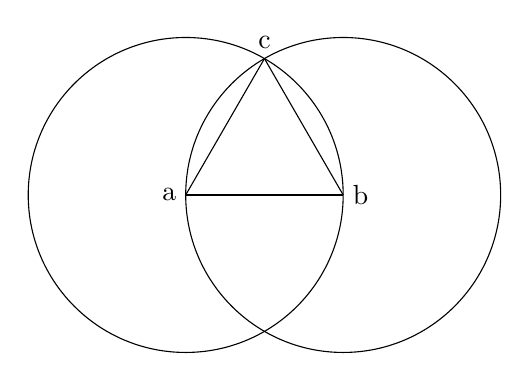
\begin{tikzpicture}
    \draw (-1,0) circle (2) node [anchor=east] {a};
	\draw (1,0) circle (2);
	\draw (-1,0) -- (1,0) node [anchor=west] {b};
	\draw (-1,0) -- (0,1.7321) node [anchor=south] {c};
	\draw (0,1.7321) -- (1,0);
\end{tikzpicture}
\caption{Построение равностороннего треугольника}
\end{figure}

Вроде бы вполне себе наглядное и очевидное доказательство, какие к нему могут быть вопросы? На самом деле это доказательство некорректно. Если вместо рассуждений на пальцах начать рассуждать более строго (например, на языке логики или около того), то окажется, что у нас возникнет проблема: мы не сможем никак доказать, что окружности с центрами в точках $a$ и $b$ вообще пересекутся. Это кажется очевидно нашей интуиции, но из сформулированных аксиом доказать этого не получится. Когда мы сталкиваемся с ситуацией, когда мы не можем доказать ни утверждение, ни его отрицание, вариантов тут может быть три:

\begin{enumerate}
\item мы просто не смогли найти пока доказательство, так как это может быть сложно;
\item что-то не так с нашей логикой, возможно нам не хватает правил вывода;
\item что-то не так с нашими аксиомами, возможно их слишком мало и их надо дополнить.
\end{enumerate}

Я сразу могу сказать, забегая вперед, что в случае евклидовой геометрии проблема именно в аксиомах: их недостаточно. Пока мы не сможем этого доказать, но мы к этой теме еще вернемся в последующих главах.

Уточним теперь понятие <<что-то не так>>. Для примера введём такую систему аксиом:

\begin{enumerate}
\item Любые две прямые пересекаются ровно в одной точке;
\item Через любые две точки проходит ровно одна прямая;
\item Существуют четыре точки такие, что они не лежат на одной прямой.
\end{enumerate}

Это довольно расплывчатые и странные аксиомы. Например, первая аксиома утверждает, что параллельных прямых не существует. Тем не менее эти аксиомы не лишены смысла. Их можно интерпретировать, например, как аксиомы геометрии, которую мы наблюдаем на плоских изображениях (фото, картины) пространства. На фото возникает это странное свойство: любые две прямые пересекаются~(см.~рис.~1.2). Если рассмотреть, например, фото железной дороги, уходящей за горизонт, то на картинке две колеи сольются на горизонте в одну точку. В физическом мире они конечно не сливаются, но фотография создаст иллюзию этого. Такая геометрия (называемая в науке проективной) вполне имеет право на существование, и очень широко применяется, например, в компьютерной трехмерной графике, не говоря уже о чисто научных применениях.

\begin{figure}[H]
\centering
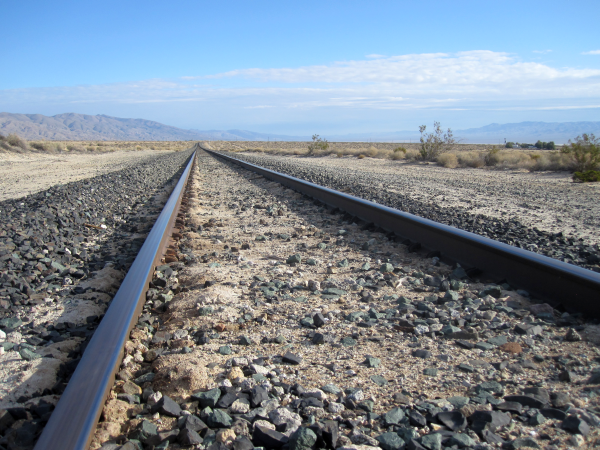
\includegraphics[width=10cm]{images/parallels.png}
\caption{В бесконечности прямые пересекаются на фото}
\end{figure}

\begin{figure}[H]
\centering
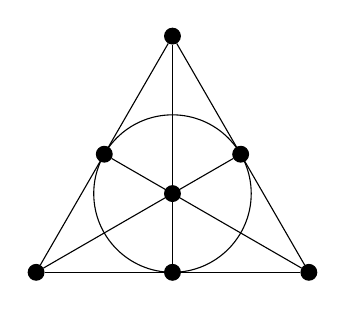
\begin{tikzpicture}
	\def\point{node [circle, draw, fill, inner sep = 0, minimum size = .2cm] }
	\draw (0, 0) \point (p1) {};
	\draw (0, -1cm) \point (p2) {};
	\draw (-.866cm, .5cm) \point (p3) {};
	\draw (.866cm, .5cm) \point (p4) {};
	\draw (-1.732cm, -1cm) \point (p5) {};
	\draw (1.732cm, -1cm) \point (p6) {};
	\draw (0, 2cm) \point (p7) {};

	\draw (0, 0) circle [radius = 1cm] {};
	\draw (p5) -- (p7);
	\draw (p6) -- (p7);
	\draw (p5) -- (p6);
	\draw (p5) -- (p4);
	\draw (p6) -- (p3);
	\draw (p2) -- (p7);
\end{tikzpicture}
\caption{Плоскость Фано}
\end{figure}

С другой стороны, мы можем отойти от привычного интуитивного определения линий и пространства, и рассмотреть конструкцию, изображенную на~рис.1.3, которая называется плоскостью Фано. Эта <<плоскость>> состоит всего из семи точек и семи линий. Каждая линия состоит из трёх точек. Очевидно, что такое построение не имеет ничего общего с первой нашей интерпретацией в виде фотографий (и даже с нашей интуицией о пространстве и линиях в нём), но простым перебором всех возможных вариантов легко убедиться, что эта <<плоскость Фано>> удовлетворяет всем трём нашим аксиомам.

Рассматривая теперь плоскость Фано и фотографию, мы можем обнаружить, что хотя эти две картинки совершенно не похожи друг на друга, у них есть общие теоремы. Один такой простейший пример демонстрирует следующее упражнение:

\begin{exercise}
Докажите, что из сформулированных аксиом можно вывести, что существуют четыре линии, не пересекающиеся в одной точке.
\end{exercise}

Есть, однако, и утверждения, которые в различных интерпретациях будут отличаться. Самое очевидное касается количества точек: на фотографии их бесконечно много, а вот на плоскости Фано их всего семь. А раз какое-то утверждение может быть либо верным, либо неверным в зависимости от интерпретации, то мы можем понять, что это утверждение из заданных аксиом вывести невозможно.

Схожим образом мы докажем в дальнейшем и невозможность доказательства первой теоремы Евклида из его аксиом: мы предъявим две интерпретации его аксиом, и в одной интерпретации близколежащие окружности будут пересекаться, а в другой нет. Это очень важный приём, так как он даёт нам однозначный ответ на вопрос о том, что это именно наши аксиомы неполны, а не что-то ещё. Мы готовы сформулировать теперь такие определения:

\begin{definition}
Система аксиом называется \term{неполной}, если существует предложение $\phi$ такое, что из аксиом невозможно вывести ни $\phi$ ни $\neg\phi$.
\end{definition}

\begin{definition}
Система аксиом называется \term{полной}, если для любого предложения $\phi$ можно вывести либо $\phi$, либо $\neg\phi$.
\end{definition}

Опять же, забегая вперёд, могу порадовать читателя: практически все полезные аксиоматические системы являются неполными. Об этом будет сказано в третьей главе, и мы даже докажем, что простейшая школьная арифметика не полна и полной быть никак не может (мы даже предъявим целый набор теорем, которые невозможно ни доказать ни опровергнуть).

В каждой конкретной интерпретации любое предложение либо истинно, либо ложно и это не зависит от возможности это доказать. Может быть такое, что у аксиом существуют разные фактически интерпретации, но при этом в них наборы истинных и ложных утверждений совпадают. Это даёт нам основание для того, чтобы в некоторых случаях рассматривать лишь такие наборы утверждений в отрыве от самой интерпретации:

\begin{definition}
\term{Структурой} называется такое множество предложений $X$, что для любого предложения $p$ либо $p\in X$, либо $\neg p \in X$.
\end{definition}

Структуры могут быть интересны иногда сами по себе и связаны с рядом задач (например, по заданной структуре найти аксиомы, которые её породили, желательно автоматически с помощью компьютера), но нами будут использоваться лишь в неотрывной связи с конкретными теориями. Желание увязать структуру с теорией приводит к следующему определению:

\begin{definition}
\term{Моделью} теории $T$ называется такая структура $M$, что для любого $p\in T$ верно, что $p\in M$. Множество всех моделей теории $T$ обозначается как $\Mod T$.
\end{definition}

\begin{definition}
Теория называется \term{удовлетворимой}, если она обладает моделью. В противном случае она называется \term{неудовлетворимой}.
\end{definition}

Разные интерпретации могут обладать одной моделью, если в них верны одинаковые предложения, а вот модель полностью определяется набором своих истинных предложений. Для неполной теории могут существовать различные модели, в которых различные предложения истинны.

Однако, даже если теория полна, это не значит, что мы можем любое истинное утверждение в ней доказать. Подходы к определению истинности высказывания, основанные на возможности доказать теорему и на возможных моделях теории, приводят к таким различным определениям:

\begin{definition}
Предложение $p$ называется \term{синтаксически истинным} в теории $T$ (обозначение $T\vdash p$), если его возможно вывести в данной теории пользуясь правилами вывода.
\end{definition}

\begin{definition}
Предложение называется \term{семантически истинным} в теории $T$ (обозначение $T\models p$), если оно истинно в любой модели данной теории.
\end{definition}

Если предложение семантически истинно, то вовсе не обязательно мы сможем это доказать правилами вывода, это зависит от того, какие собственно говоря, правила вывода мы используем. Правила вывода мы можем взять различные, и они будут обладать различными свойствами, из которых всегда хочется доказать следующее:

\begin{definition}
Набор правил вывода называется \term{полным}, если из семантической истинности предложения следует его синтаксическая истинность.
\end{definition}

Обычно в качестве правил вывода используется правило дедукции, приведенное выше, набор утверждений о логических связках, приведенных нами в первом параграфе, а также четыре правила для кванторов: обобщение и переход к частному для кванторов $\forall$ и $\exists$. Последние правила относительно сложны и мы сформулируем их строго в~\S~1.7, пока что можно думать о них интуитивно как в начале этого параграфа.

\begin{GodelsCompleteness}
Указанный набор правил вывода полон.
\end{GodelsCompleteness}

Обратите внимание на два различных термина: полный набор правил вывода и полный набор аксиом. Первый говорит о выводимости всех истинных семантических предложений  и характеризует нашу логику, которой мы пользуемся, а второй говорит не о логике, а об аксиоматической системе. Это часто вносит путаницу. Например, существуют две теоремы с похожими названиями: сформулированная нами теорема Гёделя о полноте и теорема Гёделя о \term{неполноте}. Первая говорит о том, что логика, используемая нами, в некотором смысле действительно хороша для доказательства истинных утверждений, а вторая говорит уже о неполноте аксиом арифметики. Несмотря на похожее название, эти теоремы относятся по сути совершенно к разным областям.

Доказывать теорему о полноте мы не будем, это доказательство довольно нетривиально (хоть принципиально и не сложно) и выходит за рамки данной книги. Вы можете найти его в любом подробном учебнике по логике либо в статьях в Интернете. Для практических нужд достаточно лишь знать ту логику, о которой мы до сих пор говорили, и о возможной неполноте отдельных формальных систем не задумываться, хотя чистые математики рассматривают и другие виды логики. В качестве примера в следующем параграфе мы рассмотрим модальную и темпоральную логику.

Многие операции, которые мы до сих пор рассматривали с точки зрения таблиц истинности и синтаксиса, можно так же рассмотреть и с точки зрения семантики.  В качестве примера возьмём импликацию:

\begin{definition}
Операцией импликации $p\to q$ называется такая операция, истинность которой эквивалентна выражению $\Mod(T, q)\subset\Mod(T, p)$.
\end{definition}

Здесь под $\Mod(T, p)$ понимается множество всех моделей теории $T$, дополненной предложением $p$.

\begin{exercise}
Докажите, что приведённое утверждение порождает ровно те же значения истинности, которые мы приводили в~\S1.1.
\end{exercise}

Прежде чем двинуться дальше, введем последнее простое, но важное, определение.

\begin{definition}
Теория называется противоречивой, если в ней выводимы одновременно некоторое высказывание $p$ и $\neg p$. В противном случае теория называется \term{непротеворечивой}.
\end{definition}

\begin{thm}
В противоречивой теории любое предложение синтаксически истинно.
\end{thm}
\begin{proof}
Пусть мы вывели $p$ и $\neg p$ и хотим вывести $q$. Из истинности $p$ вытекает истинность $p\lor q$ (для истинности <<или>> достаточно, чтобы истинным было одно из двух высказываний, а первое высказывание, как мы знаем, истинно). Однако теперь из того, что истинно $\neg p$ и $p\lor q$ мы получаем, что истинно так же и $q$.
\end{proof}

Это довольно странно выглядит, но на самом деле это нормально: противоречивая теория на то и противоречивая, что она не соотстветствует здравому смыслу. Очевидно так же, что противоречивая теория не может иметь модели, а следовательно и интерпретации. При построении аксиоматических систем мы должны всеми силами стараться доказать, что аксиоматика, с которой мы работаем, не протеворечива. Опять же, я могу заранее обрадовать читателя: вторая теорема Гёделя о неполноте утверждает, что для большинства полезных аксиоматик непротиворечивость доказать невозможно. Об этом мы кратко поговорим в третьей главе.

То что противоречивая теория не может иметь модели~--- это довольно очевидно. А верно ли обратное? То есть верно ли, что если нам известно, что теория модели не имеет, то она противоречива? Можно так же поставить схожий вопрос: если известно, что теория обладает единственной моделью, то верно ли, что она полна? (То что полная теория имеет единственную модель, опять же, вполне очевидно). В общем случае ответ на эти вопросы отрицательный. С другой стороны логика, которую мы рассматривали до сих пор (и которая, кстати, вполне достаточна для нужд других разделов математики~--- за её рамки нам ни разу выходить в дальнейшем не придётся и за пределами чистой логики что-либо кроме неё вообще редко встречается), всё же обладает этими свойствами. Подробности мы, однако, пока оставим в стороне, поскольку они не относятся напрямую к нашему повествованию.
